\documentclass[10pt,aspectratio=169]{beamer}

% ============================================================
% TEMA: Metropolis (moderno e limpo)
% Se der erro de pacote, troque as 3 linhas abaixo por:
%   \usetheme{Madrid}
%   \usecolortheme{seahorse}
% ============================================================
\usetheme{metropolis}
\usepackage{appendixnumberbeamer}

\usepackage[utf8]{inputenc}
\usepackage[T1]{fontenc}
\usepackage[brazil]{babel}
\usepackage{graphicx}
\usepackage{booktabs}
\usepackage{tabularx}
\usepackage{multirow}
\usepackage[svgnames,table]{xcolor}
\usepackage{tikz}
\usepackage{fontawesome5}

% ============================================================
% CORES INSTITUCIONAIS
% ============================================================
\definecolor{iffgreen}{RGB}{0, 120, 80}
\definecolor{iffblue}{RGB}{0, 70, 130}
\definecolor{lightgray}{RGB}{245, 245, 245}

\setbeamercolor{frametitle}{bg=iffblue, fg=white}
\setbeamercolor{progress bar}{fg=iffgreen}
\setbeamercolor{title separator}{fg=iffgreen}
\setbeamercolor{alerted text}{fg=iffgreen}
\setbeamercolor{block title}{bg=iffblue!15, fg=iffblue}
\setbeamercolor{block body}{bg=iffblue!5}
\setbeamercolor{block title alerted}{bg=iffgreen!15, fg=iffgreen!80!black}
\setbeamercolor{block body alerted}{bg=iffgreen!5}

\renewcommand{\figurename}{Figura}
\renewcommand{\tablename}{Tabela}

% ============================================================
% METADADOS
% ============================================================
\title{Corretor Automático de Provas usando Inteligência Artificial}
\subtitle{Trabalho de Conclusão de Curso}
\author{Lucas Lorenzo Savino \and Maycon Mendes Fernandes}
\institute{%
  Instituto Federal de Educação, Ciência e Tecnologia Fluminense\\
  \textit{Campus} Campos Centro --- Bacharelado em Engenharia da Computação\\[4pt]
  \small Orientador: Prof.\ Dr.\ Luiz Gustavo Lourenço Moura
}
\date{Abril de 2026}
\titlegraphic{}

% Logo no canto superior direito em todos os slides
\addtobeamertemplate{frametitle}{}{%
  \begin{tikzpicture}[remember picture, overlay]
    \node[anchor=north east, yshift=2pt, xshift=-2pt] at (current page.north east)
      {
\includegraphics[height=0.7cm]{iff.png}};
  \end{tikzpicture}
}

% ============================================================
\begin{document}
% ============================================================

% ------ CAPA ------------------------------------------------
{
\begin{frame}
  \titlepage
  \begin{tikzpicture}[remember picture, overlay]
    \node[anchor=north east, xshift=-8pt, yshift=-8pt] at (current page.north east)
      {
\includegraphics[height=1.0cm]{iff.png}};
  \end{tikzpicture}
\end{frame}
}

% ------ SUMÁRIO ---------------------------------------------
\begin{frame}{Sumário}
  \setbeamertemplate{section in toc}[sections numbered]
  \begin{columns}[t]
    \begin{column}{0.48\textwidth}
      \tableofcontents[hideallsubsections, sections={1-4}]
    \end{column}
    \begin{column}{0.48\textwidth}
      \tableofcontents[hideallsubsections, sections={5-9}]
    \end{column}
  \end{columns}
\end{frame}

% ============================================================
\section{Introdução e Problema}
% ============================================================

\begin{frame}{O Problema: Correção Manual de Provas Discursivas}
  \begin{columns}[T]
    \begin{column}{0.55\textwidth}
      \textbf{Desafios da correção discursiva:}
      \begin{enumerate}
        \item \textbf{Tempo:} professores dedicam \alert{6--10 h semanais} a atividades extraclasse \cite{barbosa2021} — correção compete com planejamento e acompanhamento
        \item \textbf{Fadiga do avaliador:} dificuldade de manter o mesmo rigor ao longo de muitas correções
        \item \textbf{Subjetividade:} diferentes avaliadores atribuem notas distintas à mesma resposta \cite{borges2017}
        \item \textbf{Escala:} em turmas grandes ou avaliações nacionais, o custo operacional é significativo
      \end{enumerate}
    \end{column}
    \begin{column}{0.41\textwidth}
      \begin{alertblock}{Pergunta de pesquisa}
        Como apoiar o professor com uma avaliação inicial \textbf{padronizada e rastreável}, alinhada aos seus critérios pedagógicos, \textbf{sem substituir} seu papel decisório?
      \end{alertblock}
    \end{column}
  \end{columns}
\end{frame}


% ============================================================
\section{Objetivos}
% ============================================================

\begin{frame}{Objetivo Geral}
  \begin{block}{}
    \large
    Desenvolver um \textbf{sistema de apoio à decisão docente} na correção de provas discursivas utilizando LLMs, apoiado pela recuperação dinâmica de contexto (RAG), produzindo avaliações preliminares consistentes e alinhadas aos critérios pedagógicos estabelecidos pelos professores --- \textbf{mantendo a decisão final sob responsabilidade do docente}.
  \end{block}
\end{frame}

\begin{frame}{Objetivos Específicos}
  \begin{enumerate}
    \item Construir um \textbf{banco de dados vetorial} a partir dos materiais didáticos fornecidos pelos professores (RAG)
    \item Desenvolver módulo de \textbf{configuração inicial} das provas com critérios avaliativos definidos pelo professor
    \item Implementar mecanismo de correção baseado em \textbf{múltiplos agentes independentes} com arbitragem condicional por divergência
    \item Disponibilizar \textbf{módulo de revisão docente} que permita revisar, ajustar e confirmar as correções realizadas pelo sistema
  \end{enumerate}
\end{frame}

% ============================================================
\section{Justificativa}
% ============================================================
\begin{frame}{Justificativa}
  \begin{columns}[T]
    \begin{column}{0.55\textwidth}
      \textbf{Por que esta solução é necessária:}
      \begin{itemize}
        \item Automatizar a \textbf{avaliação inicial} libera tempo docente para atividades de maior valor pedagógico — planejamento, feedback qualitativo, acompanhamento individualizado
        \item Critérios explícitos e consistentes \textbf{reduzem a variabilidade} entre correções, aumentando a equidade
        \item A revisão final permanece com o professor — a IA \textbf{complementa}, não substitui
        \item Ferramentas existentes não integram \textbf{critérios pedagógicos configuráveis} nem oferecem \textbf{rastreabilidade} das decisões automáticas
      \end{itemize}
    \end{column}
    \begin{column}{0.41\textwidth}
      \begin{block}{Contribuição esperada}
        Um artefato tecnológico que torna a correção discursiva mais \textbf{eficiente, consistente e auditável}, mantendo o docente no centro do processo avaliativo.
      \end{block}
    \end{column}
  \end{columns}
\end{frame}

% ============================================================
\section{Fundamentação Teórica}
% ============================================================

\begin{frame}{Avaliação Educacional e AES}
  \begin{columns}[T]
    \begin{column}{0.52\textwidth}
      \textbf{Avaliação discursiva}
      \begin{itemize}
        \item Exige análise qualitativa — não se reduz a gabarito
        \item Subjetividade é inerente, mas pode ser \textbf{reduzida} com critérios explícitos e padronizados
      \end{itemize}
      \vspace{0.5em}
      \textbf{AES --- \textit{Automated Essay Scoring}}
      \begin{itemize}
        \item Campo consolidado para correção automática de redações
        \item Modelos clássicos (BERT, RoBERTa) treinados em corpus anotados
        \item Limitação: dependem de dados rotulados em larga escala e língua/domínio específico
      \end{itemize}
    \end{column}
    \begin{column}{0.44\textwidth}
      \begin{block}{Lacuna que motivou este trabalho}
        AES tradicional não suporta \textbf{critérios pedagógicos configuráveis} nem integração ao fluxo de revisão docente — problemas que abordamos com LLMs + RAG.
      \end{block}
    \end{column}
  \end{columns}
\end{frame}

\begin{frame}{Conceitos-Chave}
  \begin{columns}[T]
    \begin{column}{0.48\textwidth}
      \begin{block}{LLM --- Large Language Models}
        Modelos baseados na arquitetura \textit{Transformer} (Vaswani et al., 2017), capazes de gerar texto coerente e contextualizado. Usamos \textbf{Gemini 2.5 Flash} (Google).
      \end{block}
      \vspace{0.4em}
      \begin{block}{RAG --- Recuperação Aumentada por Geração}
        Estratégia que fornece ao LLM trechos relevantes do material didático recuperados por similaridade vetorial, ancorando a correção ao conteúdo programático da disciplina.
      \end{block}
    \end{column}
    \begin{column}{0.48\textwidth}
      \begin{block}{Sistemas Multiagentes (SMA)}
        Múltiplos agentes independentes colaboram para uma tarefa. Aqui: dois corretores paralelos + árbitro condicional, inspirado no processo do ENEM.
      \end{block}
      \vspace{0.4em}
      \begin{block}{Engenharia de Prompt}
        Técnicas para instruir o LLM: \textbf{Role Prompting} (identidade especializada), \textbf{Chain-of-Thought} (raciocínio passo a passo) e \textbf{Groundedness} (fidelidade ao contexto RAG).
      \end{block}
    \end{column}
  \end{columns}
\end{frame}

% ============================================================
\section{Trabalhos Relacionados}
% ============================================================

\begin{frame}{Revisão Sistemática da Literatura}
  \begin{columns}[T]
    \begin{column}{0.50\textwidth}
      \textbf{Protocolo PICOC}
      \begin{itemize}
        \item Bases: ACM, IEEE, Scopus, Google Scholar
        \item Termos: \textit{automated grading}, \textit{LLM assessment}, \textit{essay scoring}
        \item Resultado: \textbf{7 estudos incluídos} após triagem
      \end{itemize}
      \vspace{0.5em}
      \textbf{Padrão encontrado nos estudos}
      \begin{itemize}
        \item Foco em métricas preditivas (QWK, Pearson)
        \item Domínio inglês/japonês, dados rotulados
        \item Pouca ênfase em integração institucional
      \end{itemize}
    \end{column}
    \begin{column}{0.46\textwidth}
      \begin{block}{Questões de pesquisa respondidas}
        \small
        \textbf{QP1:} LLMs são viáveis para correção? \textit{Sim, com prompts estruturados.}\\[0.4em]
        \textbf{QP2:} RAG melhora especificidade? \textit{Sim, especialmente em respostas parciais.}\\[0.4em]
        \textbf{QP3:} Há suporte a revisão docente? \textit{Não nos trabalhos analisados — esta é a lacuna.}
      \end{block}
    \end{column}
  \end{columns}
\end{frame}

\begin{frame}{Lacuna na Literatura e Oportunidade}
  \begin{columns}[T]
    \begin{column}{0.55\textwidth}
      \textbf{O que a literatura já faz bem:}
      \begin{itemize}
        \item Métricas de desempenho preditivo em cenários controlados
        \item Modelos de AES (\textit{Automated Essay Scoring}) para inglês/japonês
        \item Uso de LLMs para feedback em redações
      \end{itemize}
      \vspace{0.5em}
      \textbf{O que ainda falta:}
      \begin{itemize}
        \item Integração ao \textbf{fluxo real de correção docente}
        \item Rastreabilidade das decisões automatizadas
        \item Critérios pedagógicos explícitos configurados pelo professor
        \item Auditabilidade para revisão humana
      \end{itemize}
    \end{column}
    \begin{column}{0.41\textwidth}
      \begin{block}{Trabalho mais próximo}
        \textbf{SteLLA} (Qiu et al., 2025): sistema estruturado com LLMs + RAG para correção, mas sem mecanismo de arbitragem nem revisão docente integrada.
      \end{block}
    \end{column}
  \end{columns}
\end{frame}

% ============================================================
\section{Metodologia e Desenvolvimento}
% ============================================================

\begin{frame}{Visão Geral da Arquitetura}
  \begin{center}
    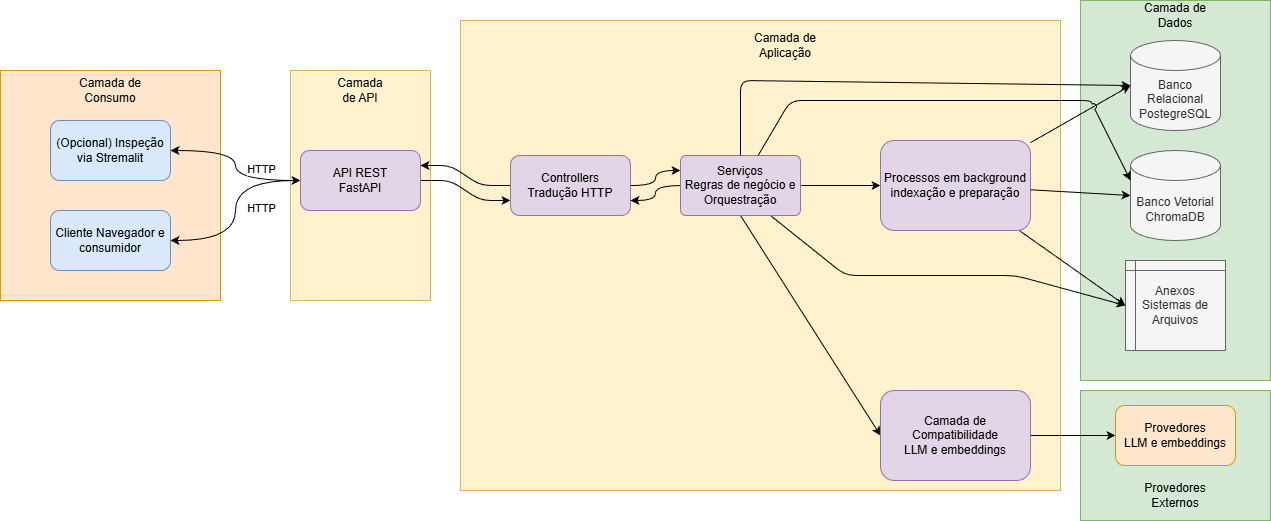
\includegraphics[width=0.90\textwidth]{diagramas/arquitetura.png}
  \end{center}
  \vspace{-0.5em}
  \begin{center}
    \small FastAPI (backend) · LangGraph (orquestração) · LangChain (agentes) · ChromaDB (vetorial) · PostgreSQL (relacional)
  \end{center}
\end{frame}

\begin{frame}{Subprocesso 1 — Configuração da Prova}
  \begin{center}
    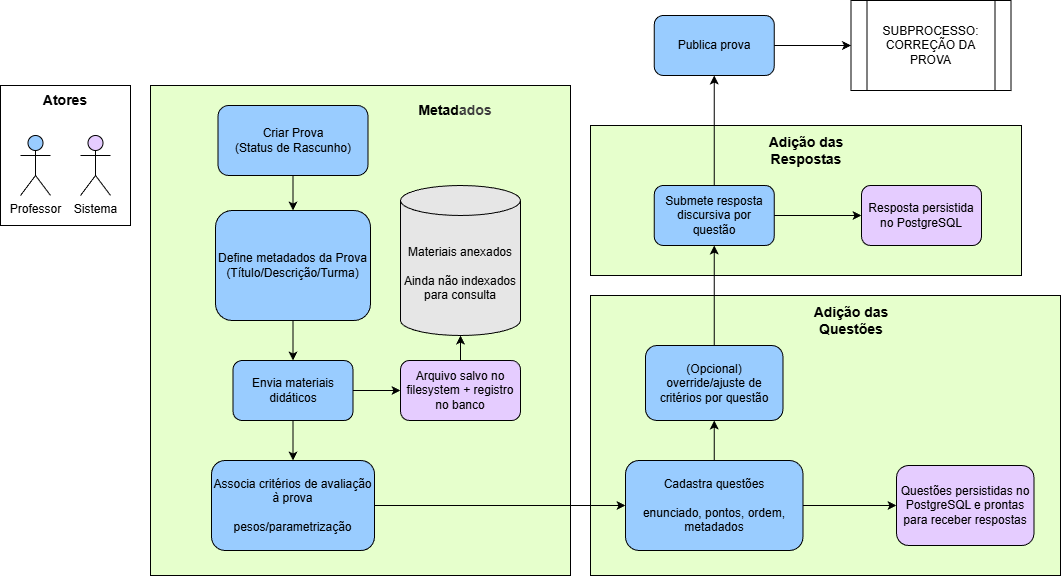
\includegraphics[width=0.80\textwidth]{diagramas/config_prova.png}
  \end{center}
\end{frame}

\begin{frame}{Subprocesso 2 — Fluxo de Correção da Prova}
  \begin{center}
    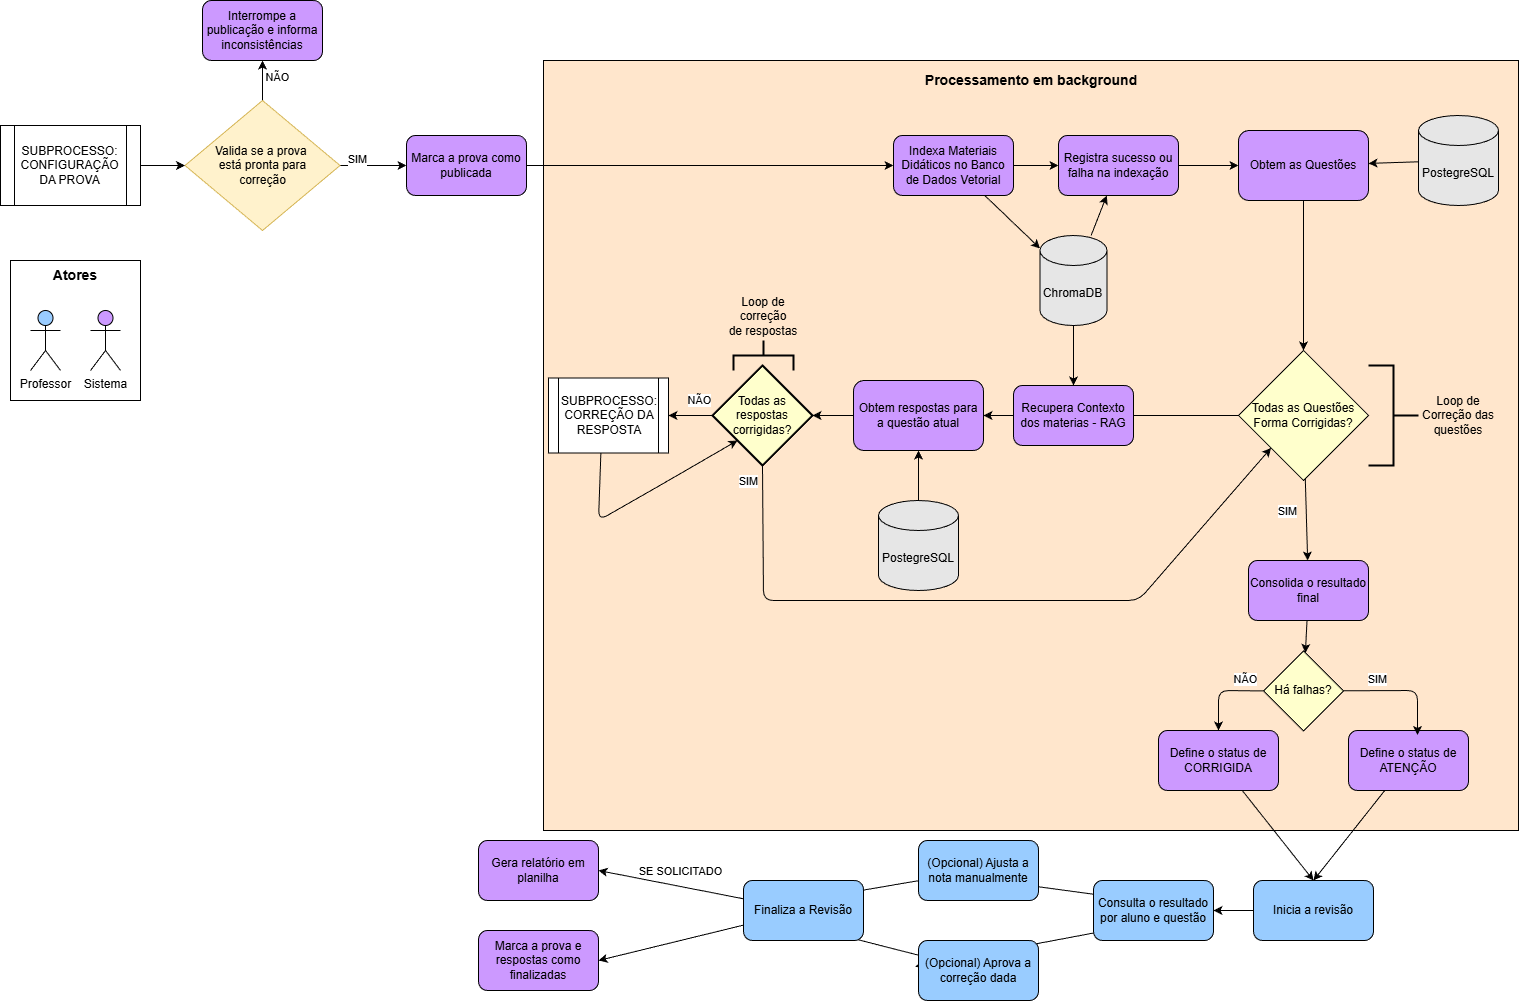
\includegraphics[width=0.78\textwidth]{diagramas/correcao_prova.png}
  \end{center}
\end{frame}

\begin{frame}{Subprocesso 3 — Fluxo de Correção da Resposta}
    \begin{center}
      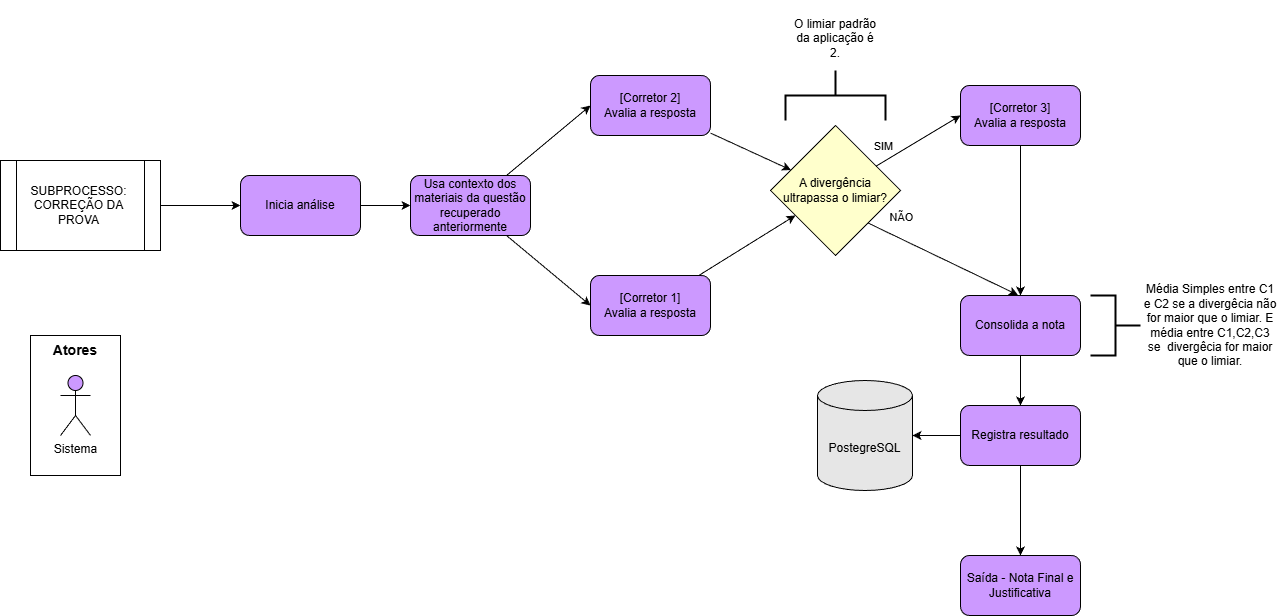
\includegraphics[width=0.90\textwidth]{diagramas/correcao_resposta.png}
    \end{center}
\end{frame}

\begin{frame}{Stack Tecnológica}
  \begin{columns}[T]
    \begin{column}{0.48\textwidth}
      \textbf{Backend e Orquestração}
      \begin{itemize}
        \item \textbf{Python + FastAPI}: API REST assíncrona
        \item \textbf{LangGraph}: grafo de estados para pipeline multiagente
        \item \textbf{LangChain}: integração com LLMs
        \item \textbf{Docker Compose}: containerização
      \end{itemize}
      \vspace{0.4em}
      \textbf{Armazenamento}
      \begin{itemize}
        \item \textbf{PostgreSQL}: dados relacionais (provas, respostas, notas)
        \item \textbf{ChromaDB}: banco vetorial para RAG
        \item \textbf{Alembic}: versionamento de esquema
      \end{itemize}
    \end{column}
    \begin{column}{0.48\textwidth}
      \textbf{IA e Modelo}
      \begin{itemize}
        \item \textbf{Gemini 2.5 Flash} (Google): LLM principal
        \item Temperatura $= 0{,}0$ (baixa estocasticidade)
        \item Embeddings para indexação vetorial
      \end{itemize}
      \vspace{0.4em}
      \textbf{Experimentação}
      \begin{itemize}
        \item \textbf{Jupyter Notebook}: orquestra experimento via API REST
        \item Resultados exportados em CSV e JSON
        \item Código disponível publicamente no GitHub
      \end{itemize}
    \end{column}
  \end{columns}
\end{frame}

% ============================================================
\section{Resultados}
% ============================================================

\begin{frame}{Desenho do Estudo}
  \begin{columns}[T]
    \begin{column}{0.52\textwidth}
      \textbf{4 Questões Avaliativas (QAs)}
      \begin{itemize}
        \item \textbf{QA1:} O sistema executa o fluxo \textit{end-to-end} sem falhas?
        \item \textbf{QA2:} O RAG melhora a especificidade da avaliação?
        \item \textbf{QA3:} O árbitro é acionado somente quando $|C1 - C2| > 2{,}0$?
        \item \textbf{QA4:} O sistema produz notas estáveis em execuções repetidas?
      \end{itemize}
    \end{column}
    \begin{column}{0.44\textwidth}
      \begin{block}{Delineamento}
        Estudo de caso controlado com \textbf{dados pareados}:\\
        Condição A (com RAG) vs. Condição B (sem RAG)\\[0.4em]
        3 questões · 4 níveis de qualidade · 12 respostas/condição
      \end{block}
      \vspace{0.4em}
      \begin{block}{Nota importante}
        \small O objetivo é validar o \textbf{funcionamento e a rastreabilidade} do sistema como artefato tecnológico de apoio ao trabalho docente --- \textbf{não} mensurar eficácia educacional ampla nem sustentar superioridade definitiva da IA sobre a correção humana.
      \end{block}
    \end{column}
  \end{columns}
\end{frame}

\begin{frame}{Configuração do Experimento}
  \begin{columns}[T]
    \begin{column}{0.50\textwidth}
      \begin{tabular}{ll}
        \toprule
        \textbf{Parâmetro} & \textbf{Valor} \\
        \midrule
        Modelo LLM & Gemini 2.5 Flash \\
        Temperatura & 0,0 \\
        Questões ($Q$) & 3 (Algoritmos e ED) \\
        Respostas por questão & 4 níveis de qualidade \\
        Total de respostas & 12 por condição \\
        Critérios de avaliação & 5 critérios \\
        Limiar de divergência & 2,0 pontos \\
        Repetições (QA4) & $R = 3$ \\
        \bottomrule
      \end{tabular}
    \end{column}
    \begin{column}{0.46\textwidth}
      \textbf{Delineamento:}
      \begin{itemize}
        \item \textbf{Condição A} (com RAG): material indexado no ChromaDB
        \item \textbf{Condição B} (sem RAG): sem material de referência
        \item \textbf{Mesmo conjunto pareado} de respostas nas duas condições
      \end{itemize}
      \vspace{0.4em}
      \textbf{Níveis de qualidade das respostas:}\\
      Excelente · Intermediária · Fraca · Fora do tema
    \end{column}
  \end{columns}
\end{frame}

\begin{frame}{QA1 — Execução \textit{End-to-End}}
  \begin{columns}[T]
    \begin{column}{0.50\textwidth}
      \begin{alertblock}{Resultado}
        \centering
        \Large \textbf{24/24 respostas processadas}\\
        \large 100\% de completude estrutural
      \end{alertblock}
      \vspace{0.5em}
      Todas as 13 etapas do fluxo concluídas com sucesso:
      \begin{itemize}
        \item Cadastro, indexação vetorial, publicação
        \item Correção paralela C1 e C2
        \item Verificação de divergência
        \item Persistência no PostgreSQL
        \item Disponibilização via API REST
      \end{itemize}
    \end{column}
    \begin{column}{0.46\textwidth}
      \textbf{Cada correção produziu:}
      \begin{itemize}
        \item Nota final consensuada
        \item Notas individuais de C1 e C2
        \item Pontuação por critério
        \item Justificativa textual por critério
        \item Valor de divergência
        \item Método de consenso aplicado
      \end{itemize}
      \vspace{0.4em}
      \begin{block}{Viabilidade técnica confirmada}
        A arquitetura multiagente com LangGraph é funcionalmente coerente e operacionalmente viável.
      \end{block}
    \end{column}
  \end{columns}
\end{frame}

\begin{frame}{QA2 — Utilidade do RAG}
  \begin{columns}[T]
    \begin{column}{0.55\textwidth}
      \begin{center}
        \small
        \begin{tabular}{lccc}
          \toprule
          \textbf{Nível} & \textbf{Média A} & \textbf{Média B} & $\boldsymbol{\Delta}$ \\
          & \textbf{(RAG)} & \textbf{(sem RAG)} & \\
          \midrule
          Excelente      & 10,00 & 10,00 & 0,00 \\
          Intermediária  & 9,31  & 8,47  & \alert{+0,84} \\
          Fraca          & 1,07  & 0,95  & +0,12 \\
          Fora do tema   & 0,00  & 0,00  & 0,00 \\
          \bottomrule
        \end{tabular}
      \end{center}
      \vspace{0.5em}
      \textbf{Maior impacto individual:}\\
      Q1/Intermediária: $\Delta = +1{,}92$ \quad Q2/Intermediária: $\Delta = +0{,}59$
    \end{column}
    \begin{column}{0.41\textwidth}
      \begin{alertblock}{Interpretação}
        O RAG funciona como \textbf{gabarito contextual}: ancora a avaliação ao conteúdo programático específico da disciplina, melhorando a precisão em respostas parcialmente corretas.
      \end{alertblock}
      \vspace{0.4em}
      Extremos inalterados: LLM identifica respostas inequívocas sem precisar de referência adicional.
    \end{column}
  \end{columns}
\end{frame}

\begin{frame}{QA3 — Arbitragem por Divergência}
  \begin{columns}[T]
    \begin{column}{0.55\textwidth}
      \begin{center}
        \small
        \begin{tabular}{lcc}
          \toprule
          \textbf{Nível} & \textbf{Divergência máx.} & \textbf{Árbitro?} \\
          \midrule
          Excelente      & 0,00 & Não \\
          Intermediária  & 1,18 & Não \\
          Fraca          & 1,22 & Não \\
          Fora do tema   & 0,00 & Não \\
          \bottomrule
        \end{tabular}
      \end{center}
      \vspace{0.3em}
      Limiar configurado: $\text{DIVERGENCE\_THRESHOLD} = 2{,}0$\\
      Divergência máxima observada: \alert{1,22 pontos}
    \end{column}
    \begin{column}{0.41\textwidth}
      \begin{block}{Critério atendido}
        Árbitro acionado \textbf{se e somente se} $|C1 - C2| > 2{,}0$. Mecanismo funcionou corretamente: nenhum acionamento indevido em 24 casos.
      \end{block}
      \vspace{0.4em}
      \textbf{Por que baixa divergência?}
      \begin{itemize}
        \item Temperatura 0,0 minimiza variabilidade
        \item Prompts com critérios explícitos
        \item Escala absoluta (0 a 10)
      \end{itemize}
    \end{column}
  \end{columns}
\end{frame}

\begin{frame}{QA4 — Estabilidade Operacional}
  \begin{columns}[T]
    \begin{column}{0.55\textwidth}
      \begin{center}
        \small
        \begin{tabular}{lcccc}
          \toprule
          \textbf{Nível} & $R_1$ & $R_2$ & $R_3$ & \textbf{Var. máx.} \\
          \midrule
          Excelente      & 10,00 & 10,00 & 10,00 & 0,00 \\
          Intermediária  & 9,88  & 9,04  & 9,08  & \alert{0,84} \\
          Fraca          & 0,51  & 1,71  & 1,88  & 1,37 \\
          Fora do tema   & 0,00  & 0,00  & 0,00  & 0,00 \\
          \bottomrule
        \end{tabular}
      \end{center}
      \vspace{0.3em}
      \small Critério: variação $\leq 1{,}0$ ponto. Questão Q2, $R=3$ repetições.
    \end{column}
    \begin{column}{0.41\textwidth}
      \textbf{Resultado:}
      \begin{itemize}
        \item Extremos: \alert{variação nula} — reprodutibilidade perfeita
        \item Intermediária: $\leq 0{,}84$ \checkmark\ (atende critério)
        \item Fraca: 1,37 (parcialmente atende)
      \end{itemize}
      \vspace{0.4em}
      \begin{block}{Nota}
        Variabilidade em respostas fracas é inerente: erros parciais coexistem com alguma terminologia adequada, gerando julgamentos ambíguos mesmo com temperatura 0,0.
      \end{block}
    \end{column}
  \end{columns}
\end{frame}

\begin{frame}{Síntese dos Resultados}
  \begin{center}
    \begin{tabular}{clll}
      \toprule
      \textbf{QA} & \textbf{Critério} & \textbf{Resultado} & \textbf{Status} \\
      \midrule
      QA1 & Completude $\geq 95\%$           & 24/24 (100\%)        & \textcolor{iffgreen}{\textbf{Atendido}} \\
      QA2 & Efeito do RAG observável         & $\Delta = +0{,}84$ (interm.) & \textcolor{iffgreen}{\textbf{Atendido}} \\
      QA3 & Árbitro acionado só se $>2{,}0$  & Máx.\ 1,22; árbitro não acionado & \textcolor{iffgreen}{\textbf{Atendido}} \\
      QA4 & Variação $\leq 1{,}0$ ponto      & Extremos: 0,00; Interm.: 0,84; Fraca: 1,37 & \textcolor{orange}{\textbf{Parcial}} \\
      \midrule
      \multicolumn{3}{l}{\textbf{Tempo de correção (12 respostas, Condição A)}} & \textbf{155 s} \\
      \bottomrule
    \end{tabular}
  \end{center}
  \vspace{0.3em}
  \begin{center}
    \small $\approx 12{,}9$ s/resposta --- tempo substancialmente inferior à correção manual
  \end{center}
\end{frame}

% ============================================================
\section{Discussão}
% ============================================================

\begin{frame}{Viabilidade Técnica e Operacional}
  \begin{columns}[T]
    \begin{column}{0.48\textwidth}
      \textbf{Viabilidade técnica}
      \begin{itemize}
        \item Fluxo \textit{end-to-end} executado sem falhas
        \item Artefatos \textbf{estruturados e rastreáveis}: nota final, notas por critério, justificativas, divergência
        \item ChromaDB + PostgreSQL integrados conforme especificado
        \item Pipeline determinístico e reproduzível
      \end{itemize}
    \end{column}
    \begin{column}{0.48\textwidth}
      \textbf{Viabilidade operacional}
      \begin{itemize}
        \item \textbf{Professor mantém autoridade}: aceita, revisa ou rejeita cada correção antes da consolidação
        \item Acesso via API REST — integrável a sistemas institucionais
        \item Corretores C1 e C2 em paralelo (LangGraph) reduzem tempo total
        \item Sistema operou de forma autônoma sem intervenção manual entre etapas
      \end{itemize}
    \end{column}
  \end{columns}
\end{frame}

\begin{frame}{Limitações Observadas}
  \begin{enumerate}
    \item \textbf{Respostas sintéticas:} conjunto de 12 respostas elaboradas pelos autores em níveis bem definidos — respostas reais têm maior variabilidade e gradações intermediárias
    \item \textbf{Escala reduzida:} 3 questões de uma única disciplina --- generalização limitada
    \item \textbf{Modelo único:} todos os experimentos com \texttt{gemini-2.5-flash} --- resultados podem variar com outros LLMs
    \item \textbf{Sem comparação com correção humana:} impossibilita mensurar acurácia absoluta (\textit{ground truth})
    \item \textbf{Árbitro não exercitado empiricamente:} nenhuma divergência ultrapassou o limiar de 2,0 pontos neste experimento
  \end{enumerate}
\end{frame}

% ============================================================
\section{Conclusão e Trabalhos Futuros}
% ============================================================

\begin{frame}{Trabalhos Futuros}
  \begin{columns}[T]
    \begin{column}{0.48\textwidth}
      \begin{itemize}
        \item \textbf{Validação com respostas humanas reais:} concordância IA vs.\ docente (coeficiente Kappa, correlação de Pearson)
        \item \textbf{Exercitação empírica do árbitro:} respostas mais heterogêneas para provocar divergências acima do limiar
        \item \textbf{Estudo multi-modelo:} OpenAI, Anthropic, modelos locais via Ollama
      \end{itemize}
    \end{column}
    \begin{column}{0.48\textwidth}
      \begin{itemize}
        \item \textbf{Análise aprofundada do RAG:} mais disciplinas e materiais didáticos
        \item \textbf{Interface docente completa:} ajuste por critério, anotações, relatórios pedagógicos de lacunas de aprendizagem
        \item \textbf{Detecção de plágio e integridade acadêmica:} similaridade entre respostas e detecção de conteúdo gerado por IA
      \end{itemize}
    \end{column}
  \end{columns}
\end{frame}

\begin{frame}{Conclusão}
  \begin{columns}[T]
    \begin{column}{0.50\textwidth}
      \textbf{Objetivos atingidos:}
      \begin{enumerate}
        \item[\checkmark] Banco vetorial (ChromaDB) construído a partir do material didático
        \item[\checkmark] Módulo de configuração com critérios e pesos definidos pelo professor
        \item[\checkmark] Correção por múltiplos agentes independentes com arbitragem condicional
        \item[\checkmark] Módulo de revisão docente integrado ao fluxo via API REST
      \end{enumerate}
    \end{column}
    \begin{column}{0.46\textwidth}
      \textbf{Resultados principais:}
      \begin{itemize}
        \item 100\% de completude \textit{end-to-end} (QA1)
        \item RAG aumentou especificidade avaliativa (QA2)
        \item Árbitro funcionou corretamente (QA3)
        \item Estabilidade satisfatória nos extremos (QA4)
      \end{itemize}
      \vspace{0.4em}
      \begin{alertblock}{}
        \small Evidência de \textbf{viabilidade técnica e operacional} — validação pedagógica com turmas reais é o próximo passo.
      \end{alertblock}
    \end{column}
  \end{columns}
\end{frame}

% ------ SLIDE FINAL -----------------------------------------
\begin{frame}[standout]
  \centering
  \Large \textbf{Obrigado!}\\[1em]
  \normalsize
  \textbf{Lucas Lorenzo Savino} \quad \textbf{Maycon Mendes Fernandes}\\[0.8em]
  Orientador: Prof.\ Dr.\ Luiz Gustavo Lourenço Moura\\[1em]
  \faGithub\quad \texttt{github.com/savinoo/ai-grading-system}\\[1em]
  \textit{Perguntas?}
\end{frame}

% ============================================================
% REFERÊNCIAS (não aparecem nos slides — apenas para \cite{})
% ============================================================
\begin{frame}[allowframebreaks]{Referências}
  \small
  \begin{thebibliography}{9}
    \bibitem{barbosa2021} BARBOSA, A. et al. Tempo de trabalho e de ensino. \textit{Educação e Pesquisa}, v. 47, 2021.
    \bibitem{borges2017} BORGES, B. G.; SILVA, S. P. D. Avaliação, exames e poderes. \textit{EDUCAÇÃO E FILOSOFIA}, v. 31, 2017.
    \bibitem{qiu2025} QIU, H. et al. SteLLA: A Structured Grading System Using LLMs with RAG. arXiv, 2025.
  \end{thebibliography}
\end{frame}

\end{document}
